\documentclass[5p,sort&compress]{elsarticle}

\usepackage{amssymb}    % Mathematical symbols
\usepackage{amsmath}    % More options for mathematics
\usepackage{subfigure}  % More options for figures
\usepackage{epstopdf}   % Convert eps to pdf
\usepackage[separate-uncertainty=true]{siunitx}   % Proper formatting of units in math mode
\usepackage{color}      % Supports text color if needed
\usepackage{soul}       % https://ctan.org/pkg/soul
\usepackage{lmodern}    % Loading fonts
\usepackage{hyperref}   % To insert clickable references/urls
\usepackage{listings}   % To input code in the text
\usepackage{amsmath}
\usepackage{amsmath}
\usepackage{amssymb}
\usepackage{graphicx}
\usepackage{epstopdf}
\usepackage{booktabs}
\setlength{\parskip}{2em}
\newcommand{\stirlingii}{\genfrac{\{}{\}}{0pt}{}}

% Choose the style of the reference list (do not change)
\bibliographystyle{elsarticle-num}

\journal{ifding/learning-notes}

% Begin the document

\begin{document}

\begin{frontmatter}
    \title{Chatper 1: Introduction}
    \author{ifding}
    
    \begin{abstract}
        Probability Theory, Decision Theory, Information Theory
    \end{abstract}


\end{frontmatter}

%% How to make a heading and divide the documents into different sections


\section{Probability Theory}

\subsection{The Rules of Probability} 

sum rule:
\begin{equation}
p(X)=\sum_{Y} p(X, Y)
\end{equation}

product rule:
\begin{equation}
p(X, Y)=p(Y | X) p(X)
\end{equation}

Here $p(X,Y)$ is a joint probability and is verbalized as ``the probability of X and Y''. $p(Y|X)$ is a conditional probability and is verbalized as ``the probability of Y given X''. $p(X)$ is a marginal probability and is simply ``the probability of X''. These two simple rules form the basis for all of the probabilistic machinery.

From the symmetry property $p(X, Y)=p(Y, X)$, we can obtain \textit{Bayes' theorem}:
\begin{equation}
p(Y | X)=\frac{p(X | Y) p(Y)}{p(X)}
\end{equation}

Using the sum rule, the denominator in Bayes' theorem can be expressed in:
\begin{equation}
p(X)=\sum_{Y} p(X | Y) p(Y)
\end{equation}

We can view the denominator in Bayes' theorem as being the normalization constant required to ensure that the sum of the conditional probability $p(Y|X)$ over all values of Y equals 1.


\subsection{Probability densities} 

Considering probabilities defined over continuous variables, If the probability of a real-valued variable $x$ falling in the interval $(x, x+ \delta x)$ is given by $p(x) \delta x$ for $\delta x \to 0$, then $p(x)$ is called the \textit{probability density} over $x$.

 \begin{figure}[h]
     \centering
     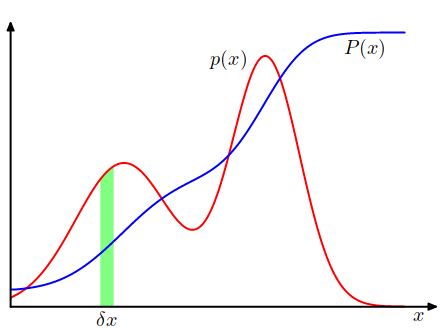
\includegraphics[width = 7.5cm]{figure/probability_density.png}
     \caption{The  probability density}
     \label{fig:1.12}
 \end{figure}

\begin{equation}
p(x \in(a, b))=\int_{a}^{b} p(x) \mathrm{d} x
\end{equation}
The probability density $p(x)$ must satisfy the two conditions:
\begin{equation}
\begin{aligned} p(x) & \geqslant 0 \\ \int_{-\infty}^{\infty} p(x) \mathrm{d} x &=1 \end{aligned}
\end{equation}

The probability that $x$ lies in the interval $(- \infty, z)$ is given by the \textit{cumulative distribution function} defined by
\begin{equation}
P(z)=\int_{-\infty}^{z} p(x) \mathrm{d} x
\end{equation}

Note that if $x$ is a discrete variable, $p(x)$ is called a \textit{probability mass function} because it can be regarded as a set of `probability masses' concentrated at the allowed values of $x$.

The sum and product rules of probability, as well as Bayes' theorem, apply equally to the case of probability densities, or to combinations of discrete and continuous variables. For instance, if x and y are two real variables,
\begin{equation}
p(x)=\int p(x, y) \mathrm{d} y
\end{equation}
\begin{equation}
p(x, y)=p(y | x) p(x)
\end{equation}

\subsection{Expectations and covariances}

One of the most important operations involving probabilities is that of finding \textbf{weighted averages} of functions. The average value of function $f(x)$ under a probability distribution $p(x)$ is called the \textit{expectation} of $f(x)$. The average is weighted by the relative probabilities of the different values of x.
\begin{equation}
\mathbb{E}[f]=\sum_{x} p(x) f(x)
\end{equation}

In the case of continuous variables, expectations are expressed by the corresponding probability density.
\begin{equation}
\mathbb{E}[f]=\int p(x) f(x) \mathrm{d} x
\end{equation}

If we are given a finite number N of points drawn from the probability distribution or probability density, then the expectation can be approximated as a finite sum over these points
\begin{equation}\label{finite_e}
\mathbb{E}[f] \simeq \frac{1}{N} \sum_{n=1}^{N} f\left(x_{n}\right)
\end{equation}

Sometimes we will be considering expectations of functions of several variables, $\mathbb{E}_{x}[f(x, y)]$ denotes the average of the function $f(x, y)$ with respect to the distribution of x. It will be a function of y. A conditional expectation with respect to a conditional distribution
\begin{equation}
\mathbb{E}_{x}[f | y]=\sum_{x} p(x | y) f(x)
\end{equation}

The \textit{variance} of $f(x)$ is defined by
\begin{equation}
\begin{aligned} \operatorname{var}[f]=\mathbb{E}\left[(f(x)-\mathbb{E}[f(x)])^{2}\right] \\ =\mathbb{E}\left[f(x)^{2}\right]-\mathbb{E}[f(x)]^{2} \end{aligned}
\end{equation}

It provides a measure of how much variability there is in $f(x)$ around its mean value $\mathbb{E}[f(x)]$.

In particular, we can consider the variance of the variable x itself, 
\begin{equation}
\operatorname{var}[x]=\mathbb{E}\left[x^{2}\right]-\mathbb{E}[x]^{2}
\end{equation}

For two random variables x and y, the \textit{covariance} is defined by
\begin{equation}
\begin{aligned} \operatorname{cov}[x, y] &=\mathbb{E}_{x, y}[\{x-\mathbb{E}[x]\}\{y-\mathbb{E}[y]\}] \\ &=\mathbb{E}_{x, y}[x y]-\mathbb{E}[x] \mathbb{E}[y] \end{aligned}
\end{equation}

which expresses the extent to which x and y vary together. If x and y are independent, then their covariance vanishes.

In the case of two vectors of random variables \textbf{x} and \textbf{y}, the covariance is a matrix
\begin{equation}
\begin{aligned} \operatorname{cov}[\mathbf{x}, \mathbf{y}] &=\mathbb{E}_{\mathbf{x}, \mathbf{y}}\left[\{\mathbf{x}-\mathbb{E}[\mathbf{x}]\}\left\{\mathbf{y}^{\mathrm{T}}-\mathbb{E}\left[\mathbf{y}^{\mathrm{T}}\right]\right\}\right] \\ &=\mathbb{E}_{\mathbf{x}, \mathbf{y}}\left[\mathbf{x} \mathbf{y}^{\mathrm{T}}\right]-\mathbb{E}[\mathbf{x}] \mathbb{E}\left[\mathbf{y}^{\mathrm{T}}\right] \end{aligned}
\end{equation}


\subsection{Bayesian probabilities}

The more general Bayesian view: probabilities provide a quantification of uncertainty. 

We can describe the uncertainty in model parameters \textbf{w}, we capture our assumptions about \textbf{w}, before observing the data, in the form of a prior probability distribution $p(\textbf{w})$.

The effect of the observed data $\mathcal{D} = \{x_1, x_2, \ldots, x_N\}$ is expressed through the conditional probability $p(\mathcal{D}|\textbf{w})$.
\begin{equation}
p(\mathbf{w} | \mathcal{D})=\frac{p(\mathcal{D} | \mathbf{w}) p(\mathbf{w})}{p(\mathcal{D})}
\end{equation}

then allows us to evaluate the uncertainty in \textbf{w} \textit{after} we have observed $\mathcal{D}$ in the form of the posterior probability $p(\textbf{w}|\mathcal{D})$.

The quantity $p(\mathcal{D}|\textbf{w})$ is evaluated for the observed data set $\mathcal{D}$ and can be viewed as a function of the parameter vector \textbf{w}, it is called the \textit{likelihood function}. It expresses how probable the observed data set is for different settings of the parameter vector \textbf{w}. 
\begin{equation}
\text { posterior } \propto \text { likelihood } \times \text { prior }
\end{equation}

where all of these quantities are viewed as functions of \textbf{w}. $p(\mathcal{D})$ is the normalization constant, which ensures that the posterior distribution is a valid probability density and integrates to one.
\begin{equation}
p(\mathcal{D})=\int p(\mathcal{D} | \mathbf{w}) p(\mathbf{w}) \mathrm{d} \mathbf{w}
\end{equation}

\textit{maximum likelihood}: \textbf{w} is set to the value that maximizes the likelihood function $p(\mathcal{D}|\textbf{w})$. This corresponds to choosing the value of $\textbf{w}$ for which the probability of observed data set is maximized. The negative log of the likelihood function is called an \textit{error function}. Maximizing the likelihood is equivalent to minimizing the error.

\subsection{The Gaussian distribution}

For the case of a single real-valued variable x, the Gaussian distribution is defined by
\begin{equation}
\mathcal{N}\left(x | \mu, \sigma^{2}\right)=\frac{1}{\left(2 \pi \sigma^{2}\right)^{1 / 2}} \exp \left\{-\frac{1}{2 \sigma^{2}}(x-\mu)^{2}\right\}
\end{equation}

which is governed by two parameters: $\mu$, called the \textit{mean}, and $\sigma^2$, called the \textit{variance}. $\sigma$ is called the \textit{standard deviation} and $\beta=1/\sigma^2$ is called the \textit{precision}.


\begin{equation}
\int_{-\infty}^{\infty} \mathcal{N}\left(x | \mu, \sigma^{2}\right) \mathrm{d} x=1
\end{equation}

The average value of x is given by
\begin{equation}
\mathbb{E}[x]=\int_{-\infty}^{\infty} \mathcal{N}\left(x | \mu, \sigma^{2}\right) x \mathrm{d} x=\mu
\end{equation}

For the second order moment
\begin{equation}
\mathbb{E}\left[x^{2}\right]=\int_{-\infty}^{\infty} \mathcal{N}\left(x | \mu, \sigma^{2}\right) x^{2} \mathrm{d} x=\mu^{2}+\sigma^{2}
\end{equation}

It follows that the variance of x is given by
\begin{equation}
\operatorname{var}[x]=\mathbb{E}\left[x^{2}\right]-\mathbb{E}[x]^{2}=\sigma^{2}
\end{equation}

Gaussian distribution over a D-dimensional vector \textbf{x} of continuous variables:
\begin{equation}
\begin{aligned}\mathcal{N}(\mathbf{x} | \boldsymbol{\mu}, \mathbf{\Sigma})= \\
\frac{1}{(2 \pi)^{D / 2}} \frac{1}{|\mathbf{\Sigma}|^{1 / 2}} \exp \left\{-\frac{1}{2}(\mathbf{x}-\boldsymbol{\mu})^{\mathrm{T}} \mathbf{\Sigma}^{-1}(\mathbf{x}-\boldsymbol{\mu})\right\}\end{aligned}
\end{equation}

where the $D$-dimensional vector $\mu$ is called the mean, the $D \times D$ matrix $\mathbf{\Sigma}$ is called the covariance, and $|\mathbf{\Sigma}|$ denotes the determinant of $\mathbf{\Sigma}$.

\begin{figure}[h]
    \centering
    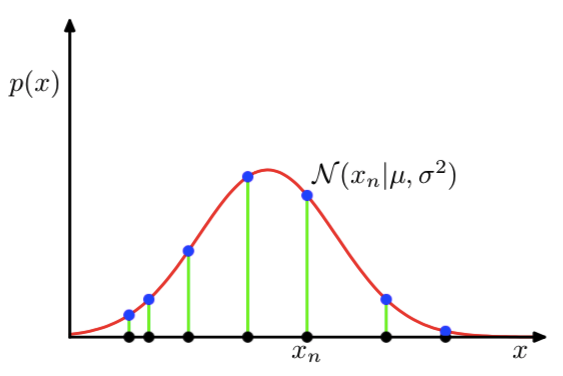
\includegraphics[width=7.5cm]{figure/gaussian.png}
    \caption{The likelihood function ($p(\mathcal{D}|\textbf{w})$) for a Gaussian distribution, shown by the red curve. Here the black points denote a data set of values $\{x_n\}$.}
    \label{fig:1.13}
\end{figure}

A data set of observations $\mathbf{X}=\left(x_{1}, \ldots, x_{N}\right)^{\mathrm{T}}$, representing N observations of the scalar variable x. \textbf{x} denotes a single observation of the vector-valued variable $\left(x_{1}, \ldots, x_{D}\right)^{\mathrm{T}}$. Our data set $\mathbf{X}$ is \textit{independent and identically distributed}, which is often abbreviated to i.i.d. 
\begin{equation}
p\left(\mathbf{X} | \mu, \sigma^{2}\right)=\prod_{n=1}^{N} \mathcal{N}\left(x_{n} | \mu, \sigma^{2}\right)
\end{equation}

As shown in Figure~\ref{fig:1.13}, the likelihood function given by the above equation corresponds to the product of the blue values. Maximizing the likelihood involves adjusting the mean $\mu$ and variance $\sigma^2$ of the Gaussian so as to maximize this product. The log likelihood function can be written in the form
\begin{equation}
\begin{aligned}{}\ln p\left(\mathbf{x} | \mu, \sigma^{2}\right) =\\
-\frac{1}{2 \sigma^{2}} \sum_{n=1}^{N}\left(x_{n}-\mu\right)^{2}-\frac{N}{2} \ln \sigma^{2}-\frac{N}{2} \ln (2 \pi)
\end{aligned}
\end{equation}

We obtain the maximum likelihood solution given by
\begin{equation}
\mu_{\mathrm{ML}}=\frac{1}{N} \sum_{n=1}^{N} x_{n}
\end{equation}
which is the sample mean i.e., the mean of the observed values $\{x_n\}$.

We obtain the maximum likelihood solution for the variance in the form
\begin{equation}
\sigma_{\mathrm{ML}}^{2}=\frac{1}{N} \sum_{n=1}^{N}\left(x_{n}-\mu_{\mathrm{ML}}\right)^{2}
\end{equation}

The \textbf{significant limitations} of the maximum likelihood approach: the maximum likelihood approach systematically underestimates the variance of the distribution. A phenomenon called \textit{bias} and \textit{overfitting}.

The maximum likelihood solutions $\mu_{ML}$ and $\sigma^2_{ML}$ are functions of the data set values $x_1, \ldots, x_N$. Consider the expectations of these quantities, 
\begin{equation}
\begin{aligned} \mathbb{E}\left[\mu_{\mathrm{ML}}\right] &=\mu \\ \mathbb{E}\left[\sigma_{\mathrm{ML}}^{2}\right] &=\left(\frac{N-1}{N}\right) \sigma^{2} \end{aligned}
\end{equation}
so that on average the maximum likelihood estimate will obtain the correct mean but will underestimate the true variance by a factor $(N-1)/N$.

As shown in Figure~\ref{fig:1.15}, the green curve shows the true Gaussian distribution from which data is generated, the three red curves show the Gaussian distributions obtained by fitting to three data sets, each consisting of two data points shown in blue. Averaged across the three data sets, the mean is correct, but the variance is systematically under-estimated because it is measured relative to the sample mean and not relative to the true mean.
\begin{figure}
    \centering
    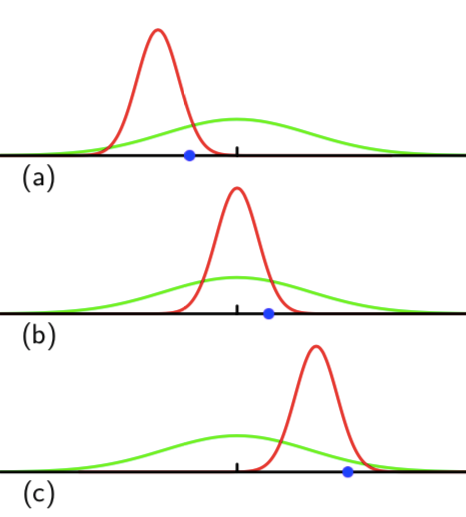
\includegraphics[width=7.5cm]{figure/mle_bias.png}
    \caption{Illustration of how bias arises in using maximum likelihood to determine the variance of a Gaussian.}
    \label{fig:1.15}
\end{figure}

Note that the bias of the maximum likelihood solution becomes less significant as the number N of data points increases. For the more complex models, the bias problems associated with maximum likelihood will be much more severe. The issue of bias in maximum likelihood lies at the root of the over-fitting problem.


\section{Decision Theory} 

Suppose we have an input vector \textbf{x} together with a corresponding vector \textbf{t} of target variables, and our goal is to predict \textbf{t} given a new value for \textbf{x}. For regression problems, \textbf{t} will comprise continuous variables. For classification problems, \textbf{t} will represent class labels.

The joint probability distribution $p(\textbf{x}, \textbf{t})$ provides a complete summary of the uncertainty associated with these variables. Determination of $p(\textbf{x}, \textbf{t})$ from a set of training data is an example of \textit{inference}.

Consider, for example, when we obtain the X-ray image \textbf{x}, our goal is to decide which of the two classes to assign to the image. We are interested in the probabilities of the two classes given the image $p(\mathcal{C}_k|\textbf{x})$.
\begin{equation}
p\left(\mathcal{C}_{k} | \mathbf{x}\right)=\frac{p\left(\mathbf{x} | \mathcal{C}_{k}\right) p\left(\mathcal{C}_{k}\right)}{p(\mathbf{x})}
\end{equation}

Here, $p(\mathcal{C}_k)$ as the prior probability for the class $\mathcal{C}_k$, and $p(\mathcal{C}_k|\textbf{x})$ as the corresponding posterior probability. If our aim is to minimize the chance of assigning \textbf{x} to the wrong class, then intuitively we would choose the class having the higher posterior probability.

We need to divide the input space into \textit{decision regions} $\mathcal{R}_k$, one for each class, such that all points in $\mathcal{R}_k$ are assigned to class $\mathcal{C}_k$.
\begin{equation}
\begin{aligned} p(\text { mistake }) &=p\left(\mathbf{x} \in \mathcal{R}_{1}, \mathcal{C}_{2}\right)+p\left(\mathbf{x} \in \mathcal{R}_{2}, \mathcal{C}_{1}\right) \\ &=\int_{\mathcal{R}_{1}} p\left(\mathbf{x}, \mathcal{C}_{2}\right) \mathrm{d} \mathbf{x}+\int_{\mathcal{R}_{2}} p\left(\mathbf{x}, \mathcal{C}_{1}\right) \mathrm{d} \mathbf{x} \end{aligned}
\end{equation}

If $p\left(\mathbf{x}, \mathcal{C}_{1}\right) > p\left(\mathbf{x}, \mathcal{C}_{2}\right)$ for a given value of \textbf{x}, then we should assign that \textbf{x} to class $\mathcal{C}_1$. 
Because $p\left(\mathbf{x}, \mathcal{C}_{k}\right)=p\left(\mathcal{C}_{k} | \mathbf{x}\right) p(\mathbf{x})$, the factor $p(\mathbf{x}$ is common to both terms.
\begin{figure}
    \centering
    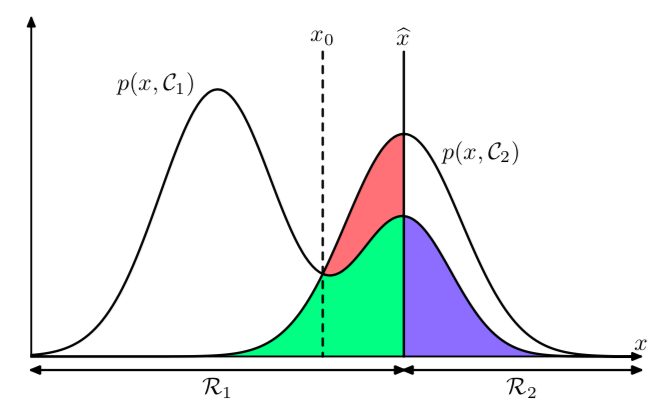
\includegraphics[width=7.5cm]{figure/decision_boundary.png}
    \caption{The joint probabilities $p\left(\mathbf{x}, \mathcal{C}_{k}\right)$ for each of two classes, with the decision boundary $x=\hat{x}$, Errors arise from the blue, green, and red regions.}
    \label{fig:1.24}
\end{figure}

In Figure~\ref{fig:1.24}, values of $x \geq \hat{x}$ are classified as $\mathcal{C}_2$, whereas they are classified as $\mathcal{C}_1$. For $x < \hat{x}$, the errors are due to points from class $\mathcal{C}_2$ being misclassified as $\mathcal{C}_1$ (the red and green regions).In the region $x \geq \hat{x}$, the errors are due to points from class $\mathcal{C}_1$ being misclassified as $\mathcal{C}_2$ (the blue region). As changing the location of $\hat{x}$, the combined areas of the green and blue regions remains constant, whereas the size of the red region varies. When set $\hat{x}=x_0$, the red region disappears, this is minimum misclassification rate decision rule, which assigns each value of x to the class having the higher posterior probability $p(\mathcal{C}_k|x)$.


\section{Information Theory}
The amount of information can be viewed as the `degree of surprise' on learning the value of random variable $x$. If a highly improbable event has just occurred, we will have received more information than some very likely event has just occurred.
\begin{equation}
h(x)=-\log _{2} p(x)
\end{equation}

where the negative sign ensures that information is positive or zero. Note that low probability events $x$ correspond to high information content. The \textit{entropy} of the discrete random variable $x$:
\begin{equation}
\mathrm{H}[x]=-\sum_{x} p(x) \ln{p(x)}
\end{equation}

Note that $\lim _{p \rightarrow 0} p \ln p=0$ and so $p(x)\ln{p(x)} = 0$. For continuous variables, the differential entropy is given by
\begin{equation}
\mathrm{H}[\mathbf{x}]=-\int p(\mathbf{x}) \ln p(\mathbf{x}) \mathrm{d} \mathbf{x}
\end{equation}

Suppose we have a joint distribution $p(\mathbf{x}, \mathbf{y})$ from which we draw pairs of values of $\mathbf{x}$ and $\mathbf{y}$. If a value of $\mathbf{x}$ is already known, then the additional information needed to specify the corresponding value of $\mathbf{y}$ is given by $\ln{p(\mathbf{y} | \mathbf{x})}$. Thus the average additional information needed to specify $\mathbf{y}$ (\textit{conditional entropy}) can be written as
\begin{equation}
\mathrm{H}[\mathbf{y} | \mathbf{x}]=-\iint p(\mathbf{y}, \mathbf{x}) \ln p(\mathbf{y} | \mathbf{x}) \mathrm{d} \mathbf{y} \mathrm{d} \mathbf{x}
\end{equation}
\begin{equation}
\mathrm{H}[\mathbf{x}, \mathbf{y}]=\mathrm{H}[\mathbf{y} | \mathbf{x}]+\mathrm{H}[\mathbf{x}]
\end{equation}

where $\mathrm{H}[\mathbf{x}, \mathbf{y}]$ is the differential entropy of $p(x,y)$ and $H[\mathbf{x}]$ is the differential entropy of the marginal distribution $p(\mathbf{x})$.


\subsection{KL divergence}

Consider some unknown distribution $p(\mathbf{x})$, and suppose that we have modelled this using an approximating distribution $q(\mathbf{x})$.
\begin{equation}
\begin{aligned} \mathrm{KL}(p \| q) &=-\int p(\mathbf{x}) \ln q(\mathbf{x}) \mathrm{d} \mathbf{x}-\left(-\int p(\mathbf{x}) \ln p(\mathbf{x}) \mathrm{d} \mathbf{x}\right) \\ &=-\int p(\mathbf{x}) \ln \left\{\frac{q(\mathbf{x})}{p(\mathbf{x})}\right\} \mathrm{d} \mathbf{x} \end{aligned}
\end{equation}

This is known as the \textit{relative entropy} or \textit{KL divergence}, between the distributions $p(\mathbf{x})$ and $q(\mathbf{x})$. Note that it is not a symmetrical quantity, KL$(p||q) \neq$  KL$(q||p)$. 

KL$(p||q) \geq 0$, if and only if, $p(\mathbf{x}) = q(\mathbf{x})$. To prove it, we first introduce the concept of \textit{convex} functions.
\begin{equation}
f(\lambda a+(1-\lambda) b) \leqslant \lambda f(a)+(1-\lambda) f(b)
\end{equation}

A convex function $f(x)$ satisfies:
\begin{equation}
f\left(\sum_{i=1}^{M} \lambda_{i} x_{i}\right) \leqslant \sum_{i=1}^{M} \lambda_{i} f\left(x_{i}\right)
\end{equation}

This result is known as \textit{Jensen's inequality}. If we interpret the $\lambda_i$ as the probability distribution over a discrete variable $x$, then
\begin{equation}
f(\mathbb{E}[x]) \leqslant \mathbb{E}[f(x)]
\end{equation}

where $\mathbb{E}[\cdot]$ denotes the expectation. For continuous variables, Jensen's inequality takes the form
\begin{equation}
f\left(\int \mathbf{x} p(\mathbf{x}) \mathrm{d} \mathbf{x}\right) \leqslant \int f(\mathbf{x}) p(\mathbf{x}) \mathrm{d} \mathbf{x}
\end{equation}
\begin{equation}
\mathrm{KL}(p \| q)=-\int p(\mathbf{x}) \ln \left\{\frac{q(\mathbf{x})}{p(\mathbf{x})}\right\} \mathrm{d} \mathbf{x} \geqslant-\ln \int q(\mathbf{x}) \mathrm{d} \mathbf{x}=0
\end{equation}

We can interpret the KL divergence as a measure of the distance of the two distributions $p(\mathbf{x})$ and $q(\mathbf{x})$.

Suppose that data is being generated from an unknown distribution $p(\mathbf{x})$ that we wish to model. We can try to approximate this distribution using some parametric distribution $q(\mathbf{x} | \theta)$, governed by a set of adjustable parameters $\mathbf{\theta}$, for example a multivariate Gaussian.

One way to determine $\mathbf{\theta}$ is to minimize the KL divergence between $p(\mathbf{x})$ and $q(\mathbf{x} | \theta)$ with respect to $\mathbf{\theta}$. We cannot do this directly because we don't know $p(\mathbf{x})$. Suppose, however, that we have observed a finite set of data points $\mathbf{x}_n$, for $n = 1, \dots, N$, drawn from $p(\mathbf{x})$.

Then the expectation with respect to $p(\mathbf{x})$ can be approximated by a finite sum over these points, using Eq.~\ref{finite_e}, so that
\begin{equation}
\mathrm{KL}(p \| q) \simeq \sum_{n=1}^{N}\left\{-\ln q\left(\mathbf{x}_{n} | \boldsymbol{\theta}\right)+\ln p\left(\mathbf{x}_{n}\right)\right\}
\end{equation}

The second term on the right-hand side is independent of $\mathbf{\theta}$, and the first term is the negative log likelihood function for $\mathbf{\theta}$ under the distribution $q(\mathbf{x} | \theta)$ evaluated using the data set. Thus we see that minimizing this KL divergence is equivalent to maximizing the likelihood function.


\subsection{mutual information}

Now consider the joint distribution between two sets of variables $\mathbf{x}$ and $\mathbf{y}$ given by $p(\mathbf{x}, \mathbf{y})$. If they are independent, $p(\mathbf{x}, \mathbf{y}) = p(\mathbf{x}) p(\mathbf{y})$. If the variables are not independent, we can gain some idea of whether whey are `close' to being independent by
\begin{equation}
\begin{aligned} \mathrm{I}[\mathbf{x}, \mathbf{y}] & \equiv \mathrm{KL}(p(\mathbf{x}, \mathbf{y}) \| p(\mathbf{x}) p(\mathbf{y})) \\ &=-\iint p(\mathbf{x}, \mathbf{y}) \ln \left(\frac{p(\mathbf{x}) p(\mathbf{y})}{p(\mathbf{x}, \mathbf{y})}\right) \mathrm{d} \mathbf{x} \mathrm{d} \mathbf{y} \end{aligned}
\end{equation}

which is called the \textit{mutual information} between the variables \textit{x} and \textit{y}. $\mathrm{I}[\mathbf{x}, \mathbf{y}] \geq 0$ with equality if, and only if, \textit{x} and \textit{y} are independent.
\begin{equation}
\mathrm{I}[\mathbf{x}, \mathbf{y}]=\mathrm{H}[\mathbf{x}]-\mathrm{H}[\mathbf{x} | \mathbf{y}]=\mathrm{H}[\mathbf{y}]-\mathrm{H}[\mathbf{y} | \mathbf{x}]
\end{equation}

Thus we can view the mutual information as the reduction in the uncertainty about \textbf{x} by virtue of being told the value of \textbf{y} (or vice versa). 

From a Bayesian perspective, we can view $p(\mathbf{x})$ as the prior distribution for \textit{x} and $p(\mathbf{x} | \mathbf{y})$ as the posterior distribution after we have observed new data \textbf{y}. The mutual information therefore represents the reduction in uncertainty about \textbf{x} as a consequence of the new observation \textbf{y}.

\section{Exercises}

1.6 Based on the following equation:
\begin{equation}
\begin{aligned} \operatorname{cov}[\mathbf{x}, \mathbf{y}] &=\mathbb{E}_{\mathbf{x}, \mathbf{y}}\left[\{\mathbf{x}-\mathbb{E}[\mathbf{x}]\}\left\{\mathbf{y}^{\mathrm{T}}-\mathbb{E}\left[\mathbf{y}^{\mathrm{T}}\right]\right\}\right] \\ &=\mathbb{E}_{\mathbf{x}, \mathbf{y}}\left[\mathbf{x} \mathbf{y}^{\mathrm{T}}\right]-\mathbb{E}[\mathbf{x}] \mathbb{E}\left[\mathbf{y}^{\mathrm{T}}\right] \end{aligned}
\end{equation}

Because $\mathbf{x}$ and $\mathbf{y}$ is independent, we have:
$p(\mathbf{x}, \mathbf{y}) = p_{\mathbf{x}}(\mathbf{x})p_{\mathbf{y}}(\mathbf{y})$, therefore:
\begin{equation}
\begin{aligned} \iint x y p(x, y) d x d y &=\iint x y p_{x}(x) p_{y}(y) d x d y \\ &\left.=\left(\int x p_{x}(x) d x\right) \int y p_{y}(y) d y\right) \\=>\mathbb{E}_{x, y}[x y] &=\mathbb{E}[x][\mathrm{E}[y] => \operatorname{cov}[\mathbf{x}, \mathbf{y}] =0\end{aligned}
\end{equation}

1.10 Suppose that two variables x and z are statistically independent.
\begin{equation}
\begin{aligned} \mathbb{E}[x+z] &=\iint(x+z) p(x, z) d x d z \\ &=\iint(x+z) p(x) p(z) d x d z \\ &=\iint x p(x) p(z) d x d z+\iint z p(x) p(z) d x d z \\ &=\int\left(\int p(z) d z\right) x p(x) d x+\int\left(\int p(x) d x\right) z p(z) d z \\ &=\int x p(x) d x+\int z p(z) d z \\ &=\mathbb{E}(x]+\mathbb{E}[z] \end{aligned}
\end{equation}

\begin{equation}
\begin{aligned} \operatorname{var}[x+z] &=\iint(x+z-\mathbb{E}[x+z])^{2} p(x, z) d x d z \\ & =\iint\{(x+z)^{2}-2(x+z) \mathbb{E}[x+z]+ \\ & \mathbb{E}^{2}[x+z]\} p(x, z) d x d z \\ &=\iint(x+z)^{2} p(x, z) d x d z- \\ & 2 \mathbb{E}[x+z] \iint(x+z) p(x, z) d x d z+\mathbb{E}^{2}[x+z] \\ &=\iint\left(x^{2}+z\right)^{2} p(x, z) d x d z-\mathbb{E}^{2}[x+z] \\ &=\iint\left(x^{2}+2 x z+z^{2}\right) p(x) p(z) d x d z-\mathbb{E}^{2}[x+z] \\ &=\mathbb{E}\left[x^{2}\right]+\mathbb{E}\left[z^{2}\right]-\mathbb{E}[z]-2 \mathbb{E}[x] \mathbb{E}[z]+ \\ & 2 \iint x z p(x) p(z) d x d z \\ &=\operatorname{var}[x]+\operatorname{var}[z]-2 \mathbb{E}[x] \mathbb{E}[z]+ \\ & 2\left(\int x p(x) d x\right) \iint x z p(x) p(z) d x d z \\ &=\operatorname{var}[x]+\operatorname{var}[z] \end{aligned}
\end{equation}

1.30 Evaluate the KL divergence between two Gaussians $p(x)=\mathcal{N}\left(x | \mu, \sigma^{2}\right)$ and $q(x)=\mathcal{N}\left(x | m, s^{2}\right)$.

Based on definition:
\begin{equation}
\begin{aligned} \ln \{\frac{p(x)}{q(x)}\} &=\ln \left(\frac{s}{\sigma}\right)-[\frac{1}{2 \sigma^{2}}(x-\mu)^{2}-\frac{1}{2 s^{2}}(x-m)^{2}] \\ &=\ln \left(\frac{s}{\sigma}\right)-[\left(\frac{1}{2 \sigma^{2}}-\frac{1}{2 s^{2}}\right) x^{2} \\ & -\left(\frac{\mu}{\sigma^{2}}-\frac{m}{s^{2}}\right) x+\left(\frac{\mu^{2}}{2 \sigma^{2}}-\frac{m^{2}}{2 s^{2}}\right)] \end{aligned}
\end{equation}

We will take advantage of the following equations to solve this problem
\begin{equation}
\begin{aligned}
\mathbb{E}\left[x^{2}\right]=\int x^{2} \mathcal{N}\left(x | \mu, \sigma^{2}\right) d x=\mu^{2}+\sigma^{2} \\
\mathbb{E}[x]= \int x \mathcal{N}\left(x | \mu, \sigma^{2}\right) d x= \mu \\
\int \mathcal{N}\left(x | \mu, \sigma^{2}\right) d x=1
\end{aligned}
\end{equation}
\begin{equation}
\begin{aligned} K L(p \| q) &=-\int p(x) \ln \{\frac{q(x)}{p(x)}\} d x \\ &=\ln \left(\frac{s}{\sigma}\right)-\left(\frac{1}{2 \sigma^{2}}-\frac{1}{2 s^{2}}\right)(\mu^{2}+\sigma^{2})+ \\ & (\frac{\mu}{\sigma^{2}}-\frac{m}{s^{2}}) \mu-(\frac{\mu^{2}}{2 \sigma^{2}}-\frac{m^{2}}{2 s^{2}}) \\ &=\ln \left(\frac{s}{\sigma}\right)+\frac{\sigma^{2}+(\mu-m)^{2}}{2 s^{2}}-\frac{1}{2} \end{aligned}
\end{equation}

1.31 Based on $p(\mathbf{x}, \mathbf{y})=p(\mathbf{x}) p(\mathbf{y} | \mathbf{x}), \int p(\mathbf{x}, \mathbf{y}) d \mathbf{y}=p(\mathbf{x})$, we first calculate $H[\mathbf{x}, \mathbf{y}]$:
\begin{equation}
\begin{aligned} H[\mathbf{x}, \mathbf{y}] &=-\iint p(\mathbf{x}, \mathbf{y}) \ln p(\mathbf{x}, \mathbf{y}) d \mathbf{x} d \mathbf{y} \\ &=-\iint p(\mathbf{x}, \mathbf{y}) \ln p(\mathbf{x}) d \mathbf{x} d \mathbf{y} \\ &
-\iint p(\mathbf{x}, \mathbf{y}) \ln p(\mathbf{y} | \mathbf{x}) d \mathbf{x} d \mathbf{y} \\ &=-\int p(\mathbf{x}) \ln p(\mathbf{x}) d \mathbf{x}-\iint p(\mathbf{x}, \mathbf{y}) \ln p(\mathbf{y} | \mathbf{x}) d \mathbf{x} d \mathbf{y} \\ &=H[\mathbf{x}]+H[\mathbf{y} | \mathbf{x}] \end{aligned}
\end{equation}

$H[\mathbf{x}]+H[\mathbf{y}] -H[\mathbf{x}, \mathbf{y}]=H[\mathbf{y}]-H[\mathbf{y} | \mathbf{x}]$
\begin{equation}
\begin{aligned} \\ &=-\int p(\mathbf{y}) \ln p(\mathbf{y}) d \mathbf{y}+\iint p(\mathbf{x}, \mathbf{y}) \ln p(\mathbf{y} | \mathbf{x}) d \mathbf{x} d \mathbf{y} \\ &=-\iint p(\mathbf{x}, \mathbf{y}) \ln p(\mathbf{y}) d \mathbf{x} d \mathbf{y}+\iint p(\mathbf{x}, \mathbf{y}) \ln p(\mathbf{y} | \mathbf{x}) d \mathbf{x} d \mathbf{y} \\ &=-\iint p(\mathbf{x}, \mathbf{y}) \ln \left(\frac{p(\mathbf{x}) p(\mathbf{y})}{p(\mathbf{x}, \mathbf{y})}\right) d \mathbf{x} d \mathbf{y} \\ &=K L(p(\mathbf{x}, \mathbf{y}) \| p(\mathbf{x}) p(\mathbf{y}))=I(\mathbf{x}, \mathbf{y}) \geq 0 \end{aligned}
\end{equation}

The mutual information
\begin{equation}
I(\mathbf{x}, \mathbf{y})=-\iint p(\mathbf{x}, \mathbf{y}) \ln \left(\frac{p(\mathbf{x}) p(\mathbf{y})}{p(\mathbf{x}, \mathbf{y})}\right) d \mathbf{x} d \mathbf{y}
\end{equation}

\section*{References}
\bibliography{references}

\begin{thebibliography}{9}

\bibitem{Bishop} 
Bishop, Christopher M. Pattern recognition and machine learning. springer, 2006.

\bibitem{zhengqigao}
https://github.com/zhengqigao/PRML-Solution-Manual


\end{thebibliography}
\end{document}